\section{Experiments}\label{interpretability_crr_sec:experiment}
We implement a prototype  of  $ \crr $\footnote{The source code is available at \url{https://github.com/meelgroup/mlic}} based on the  Python API for CPLEX  and conduct an extensive  empirical analysis to understand the behavior of $\crr$ on real-world instances. The objective of our experimental evaluation is to answer the following questions:


\begin{enumerate}
	\item How do the accuracy and training time for  {\crr}  behave vis-a-vis state-of-the-art classifiers on large datasets arising in machine learning problems in practice?
	\item Can {\crr} generate sparse rules compared to that of  other rule-based models? 
	\item How do the training time, accuracy, and rule size vary with model hyper-parameters?
\end{enumerate}


In summary, relaxed-CNF rules generated by {\crr} achieves higher accuracy and more concise representation than CNF rules in most of the datasets. Moreover, relaxed-CNF rules are shown to be sparser than decision lists with competitive accuracy in large datasets.  Finally, we show how to control the trade-off between rule-sparsity and accuracy using the hyper-parameter $ \lambda $; and between accuracy and training time using the hyper-parameter $ k $ and size $ n_p $ of each mini-batch. In the following, we give a detailed description of the experiments. 



%%\vspace{-3pt}
\subsection{Experiment Methodology}
We perform experiments on a high-performance computer cluster, where each node consists of E$ 5$-$2690\text{ v}3 $ CPU with $ 24 $ cores, $ 96 $ GB of RAM. Each experiment is run on four cores of a node with $ 16 $ GB memory.   We compare the performance of  $ \crr $   with  state-of-the-art classifiers, e.g. $ \IMLI  $~\cite{GM2019}, RIPPER~\cite{C1995}, BRS~\cite{WRDLKM2017},  random forest (RF), support vector classifier (SVC), nearest neighbors classifiers ($ k $-NN), and $ l_1 $ penalized logistic regression (LR). Among them, {\IMLI}, BRS, and RIPPER are rule-based classifiers. In particular,
{\IMLI} generates classification rules in CNF using a MaxSAT-based formulation and we use Open-WBO \cite{MML2014} as the MaxSAT solver for {\IMLI}. We compare with propositional rule learning algorithm RIPPER, which is implemented in WEKA~\cite{HFHPRW2009} and generates classification rules in the form of decision lists. BRS is a Bayesian framework for generating rule sets expressed as DNF. For  other classifiers, we use the Scikit-learn module of Python~\cite{PVGMTGB2011}. For all  classifiers, we set the training cut-off time to $ 1500 $  {seconds}. 

\begin{table}
	\caption[Accuracy, rule-size, and training time of rule-based classifiers]{Comparisons of test accuracy, rule-size and training time among different rule-based classifiers. Every cell in the last four columns contains the test accuracy in percentage (top value), rule size  (middle value), and  training time in seconds (bottom value). In the experiments, {\crr} shows higher test accuracy than IMLI and generates sparser rules than RIPPER. Number in bold denotes the best result, such as maximum test accuracy, minimum rule-size, and minimum training time among competitive classifiers.}
	\label{interpretability_crr_tab:rule_based_classifiers}
	
	
%	\setlength{\tabcolsep}{3pt} 
	\begin{center}
		\begin{tabular}{l  r  r r r r r r r rrr}
			\toprule
			{{Dataset}} & Size & Features  & RIPPER & BRS & IMLI & CRR\\
			\midrule
			{ Heart}   & $  303 $  & $  31 $  & $   \textbf{78.69}  $    & $   72.13  $    & $   72.13  $    & $   77.69  $   \\ & & 
			& $   7 $    & $   19 $    & $   13 $    & $   \textbf{4.5}  $   \\ & & 
			& $   5.27 \text{s}  $    & $   25.07 \text{s}  $    & $   \textbf{1.8} \text{s}  $    & $   122.5 \text{s}  $   \\
			\midrule 
			{ Ionosphere}   & $  351 $  & $  144 $  & $   88.65  $    & $   \textbf{91.43}  $    & $   89.29  $    & $   \textbf{91.43}  $   \\ & & 
			& $   8 $    & $   \textbf{4} $    & $   8.5  $    & $   20 $   \\ & & 
			& $   5.87 \text{s}  $    & $   75.53 \text{s}  $    & $   \textbf{2.09} \text{s}  $    & $   5.59 \text{s}  $   \\
			\midrule 
			{ WDBC}   & $  569 $  & $  88 $  & $   95.22  $    & $   \textbf{95.65}  $    & $   93.91  $    & $   94.69  $   \\ & & 
			& $   7.5  $    & $   12 $    & $   \textbf{7} $    & $   34.5  $   \\ & & 
			& $   5.7 \text{s}  $    & $   630.23 \text{s}  $    & $   \textbf{1.38} \text{s}  $    & $   316.32 \text{s}  $   \\
			\midrule 
			{ Magic}   & $  19020 $  & $  79 $  & $   \textbf{84.04}  $    & $   74.15  $    & $   71.97  $    & $   81.31  $   \\ & & 
			& $   115 $    & $   \textbf{3} $    & $   24 $    & $   31 $   \\ & & 
			& $   \textbf{15.86} \text{s}  $    & $   56.46 \text{s}  $    & $   141.2 \text{s}  $    & $   1012.6 \text{s}  $   \\
			\midrule 
			{ Tom's HW}   & $  28179 $  & $  910 $  & $   \textbf{97.4}  $    &   \multicolumn{1}{c}{\multirow{3}{*}{\textemdash}}       & $   95.88  $    & $   97.34  $   \\ & & 
			& $   36 $    &       & $   30 $    & $   \textbf{4} $   \\ & & 
			& $   \textbf{42.73} \text{s}  $    &       & $   92.65 \text{s}  $    & $   1071.58 \text{s}  $   \\
			\midrule 
			{ Credit}   & $  30000 $  & $  110 $  & $   81.68  $    &   \multicolumn{1}{c}{\multirow{3}{*}{\textemdash}}       & $   81.42  $    & $  \textbf{ 82.04}  $   \\ & & 
			& $   38.5  $    &       & $   \textbf{10} $    & $   32 $   \\ & & 
			& $   \textbf{14.52} \text{s}  $    &       & $   17.66 \text{s}  $    & $   1021.35 \text{s}  $   \\
			\midrule 
			{ Adult}   & $  32561 $  & $  144 $  & $   84.31  $    &   \multicolumn{1}{c}{\multirow{3}{*}{\textemdash}}       & $   82.08  $    & $   \textbf{84.86}  $   \\ & & 
			& $   94 $    &       & $   23 $    & $   \textbf{18} $   \\ & & 
			& $   27.61 \text{s}  $    &       & $   \textbf{11.91} \text{s}  $    & $   1016.36 \text{s}  $   \\
			\midrule 
			{ Twitter}   & $  49999 $  & $  1511 $  & $   \textbf{95.74}  $    &   \multicolumn{1}{c}{\multirow{3}{*}{\textemdash}}       & $   94.24  $    & $   95.16  $   \\ & & 
			& $   179.5  $    &       & $   57 $    & $   \textbf{12} $   \\ & & 
			& $   \textbf{170.87} \text{s}  $    &       & $   238.29 \text{s}  $    & $   1144.66 \text{s}  $   \\
			\midrule 
			{ Weather-AUS}   & $  107696 $  & $  141 $  & $   \textbf{84.57}  $    &   \multicolumn{1}{c}{\multirow{3}{*}{\textemdash}}       & $   82.83  $    & $   83.34  $   \\ & & 
			& $   195 $    &       & $   7 $    & $   \textbf{2} $   \\ & & 
			& $   \textbf{121.02} \text{s}  $    &       & $   366.12 \text{s}  $    & $   1115.27 \text{s}  $   \\
			\midrule 
			{ Skin}   & $  245057 $  & $  119 $  & $   98.32  $    &   \multicolumn{1}{c}{\multirow{3}{*}{\textemdash}}       & $   \textbf{98.92}  $    & $   95.08  $   \\ & & 
			& $   725 $    &       & $   201 $    & $   \textbf{29} $   \\ & & 
			& $   1313.19 \text{s}  $    &       & $   \textbf{103.8} \text{s}  $    & $   825.6 \text{s}  $   \\
			\bottomrule
		\end{tabular}
	\end{center}
	
	
\end{table}



We consider a comparable number  of hyper-parameter choices  for each classifier. Specifically for {\crr}, we choose the data-fidelity parameter $ \lambda \in \{0.5, 0.67, 0.84, 0.99\} $, the number of clauses $ k \in \{1,2,3\} $, the relative size of mini-batch $ \frac{n_p}{n} \in \{0.25, 0.50, 0.75\} $, and the number of iterations $ \tau \in \{2,4,8,16\} $. We learn the value of $ \card_c $ and $ \eta_{l} $ from the dataset as described in Chapter.~\ref{interpretability_crr_sec:ilp_query}.  In CPLEX, we set the  maximum solving time of the LP solver to $ 1000 $  seconds ($ \frac{ 1000 }{\tau} $ seconds for each iteration) and the remaining $ 500 $ seconds is allotted to construct the MLIP instances, parse the solutions and execute  other auxiliary tasks of the learning algorithm. We present the current best solution of CPLEX when the solver times out while finding the optimal solution.  

We control the cut-off of the number of examples in the leaf node in the case of RF and RIPPER. For SVC, $ k $-NN, and LR we discretize the regularization parameter on a logarithmic grid. For BRS, we vary the max clause-length $ \in \{3,4,5\} $, support $ \in  \{5,10,15\} $, and two other parameters $ s \in \{100,1000,10000\} $ and $ \rho \in \{0.9,0.95,0.99\} $.  For  {\IMLI}, we consider  $ \lambda \in \{1,5,10\} $ and  $ k \in \{1,2,3\} $ and  vary the number of batches $ \tau $ such that each batch has at least $ 32 $ samples and at most $ 512 $ samples.  




	








%%\vspace{-9pt}
\subsection{Results}
In the following, we first discuss empirical results of rule-based classifiers, then extend analysis to non-rule-based classifiers, and finally discuss the effect of different choices of hyper-parameters. 
%%\vspace{-3pt}
\subsubsection*{Performance Evaluation of {\crr} with Rule-based Classifiers:}
We conduct an assessment of performance  using five-fold nested cross-validation as in~\cite{DGW2018}  and report the median of test accuracy, rule-size and training time of all rule-based classifiers in Table~\ref{interpretability_crr_tab:rule_based_classifiers}. 
Specifically, we show the dataset,  the number of samples and the number of discretized features in the first three columns in Table~\ref{interpretability_crr_tab:rule_based_classifiers}. Inside each cell of column   four to $    11 $,  we present the   test accuracy (top value), rule-size (middle value) and training time (bottom value) of each classifier for each dataset. 



We first compare relaxed-CNF rules generated by {\crr} with CNF rules generated by IMLI. In {Table}~\ref{interpretability_crr_tab:rule_based_classifiers}, relaxed-CNF rules exhibit higher prediction accuracy than CNF rules in the majority of the datasets, showing the effectiveness of using a more expressive representation of classification rules in capturing the decision boundary. In addition, the generated relaxed-CNF rules are comparatively smaller than CNF rules in terms of rule-size in most of the datasets. Therefore, relaxed-CNF rules improve upon CNF rules in terms of both prediction accuracy and rule size in the majority of the datasets. In this context, {\crr} provides a trade-off between accuracy and rule-size depending on the choice of hyper-parameters and the experimental results are discussed later in Section~\ref{interpretability_crr_sec:model_parameters}.  We then compare relaxed-CNF rules with DNF rules generated by BRS and find that relaxed-CNF rules outperform DNF rules with respect to prediction accuracy in several datasets. At this point,   BRS fails to scale on larger datasets as shown in Table~\ref{interpretability_crr_tab:rule_based_classifiers}. We finally compare relaxed-CNF rules with decision lists generated by RIPPER.  In the experiments, relaxed-CNF rules achieve comparable prediction accuracy with decision lists in most of the datasets. In contrast,   RIPPER generates very large decision lists compared to relaxed-CNF rules in the majority of the datasets, more precisely in large datasets.  To summarize the performance of {\crr} among different rule-based classifiers,  {\crr} can generate smaller relaxed-CNF rules with better accuracy in numbers of the cases with a couple of exceptions. 



Moving focus on the training time,  the non-incremental version of {\crr} times out on larger instances in the experiments, potentially producing sub-optimal rules with reduced accuracy, thereby highlighting the need for the incremental approach. On the other hand, the incremental version of {\crr} can handle most of the datasets within the allotted amount of time. In Table~\ref{interpretability_crr_tab:rule_based_classifiers}, {\crr} takes a comparatively longer time to generate relaxed-CNF rules in comparison with other rule-based classifiers, e.g., RIPPER, and IMLI because of  the flexible combinatorial structure of relaxed-CNF rules. However, the testing time of {\crr} is insignificant ($ < 0.01 $ seconds) and thus can 
 be deployed in practice.  
 
 
 
 
 

\subsubsection*{Performance Evaluation of {\crr} with Non-rule-based Classifiers:}

We compare  the  test accuracy of {\crr} with  non-rule-based classifiers:  LR, SVC, RF, and $ k $-NN and report the results in Table~\ref{interpretability_crr_tab:all_classifiers}. In the experiments, we  find that {\crr},  in spite of being a rule-based classifier, is able to achieve competitive prediction accuracy with non-rule-based classifiers.  In this context, SVC, and $ k $-NN  can not complete training  within the allotted time particularly in the  datasets with more than $ 10^5 $ samples, while {\crr} can still generate relaxed-CNF rules with competitive accuracy. 
Therefore, {\crr} shows the promise of applying rule-based classifiers in practice with an added benefit of interpretability along with competitive accuracy.






\begin{table}
	\caption[Accuracy of {\crr} and non-rule-based classifiers]{Comparisons of test accuracy among {\crr} and  non-rule-based classifiers. In the experiments, {\crr} achieves competitive prediction accuracy in spite of being a rule-based classifier.}
	\label{interpretability_crr_tab:all_classifiers}
	\begin{center}
		\begin{tabular}{l   r r r r r  r }
			\toprule
			{Dataset}  & LR & SVC & RF & $k$-NN & CRR\\\midrule
			\multirow{1}{*}{ Heart}   & $   \textbf{84.29}  $    & $   83.33  $    & $   81.97  $    & $   78.69  $    & $   77.69  $   \\ 
			\multirow{1}{*}{ Ionosphere}   & $   \textbf{94.29}  $    & $   91.43  $    & $   92.96  $    & $   91.43  $    & $   91.43  $   \\ 
			\multirow{1}{*}{ WDBC}   & $   \textbf{98.26}  $    & $   96.46  $    & $   96.90  $    & $   95.61  $    & $   94.69  $   \\ 
			\multirow{1}{*}{ Magic}   & $   85.15  $    & $   84.45  $    & $   \textbf{85.30}  $    & $   77.9  $    & $   81.31  $   \\ 
			\multirow{1}{*}{ Tom's HW}   & $   97.62  $    & $   \textbf{97.66}  $    & $   97.52  $    & $   94.59  $    & $   97.34  $   \\ 
			\multirow{1}{*}{ Credit}   & $   82.04  $    & $   \textbf{82.12}  $    & $   81.97  $    & $   80.5  $    & $   82.04  $   \\ 
			\multirow{1}{*}{ Adult}   & $   \textbf{87.24}  $    & $   86.82  $    & $   86.84  $    & $   84.68  $    & $   84.86  $   \\ 
			\multirow{1}{*}{ Twitter}   & $   96.28  $    & $   96.34  $    & $   \textbf{96.37}  $     &  \multicolumn{1}{c}{\textemdash}      & $   95.16  $   \\ 
			\multirow{1}{*}{ Weather-AUS}   & $   \textbf{85.71}  $     &  \multicolumn{1}{c}{\textemdash}      & $   85.63  $     &  \multicolumn{1}{c}{\textemdash}      & $   83.34  $   \\ 
			\multirow{1}{*}{ Skin}   & $   97.21  $     &  \multicolumn{1}{c}{\textemdash}      & $   \textbf{99.81}  $     &  \multicolumn{1}{c}{\textemdash}      & $   95.08  $   \\ 
			\bottomrule
		\end{tabular}
	\end{center}
\end{table}




\begin{figure}[t]
	\centering
	
	\subfloat
	{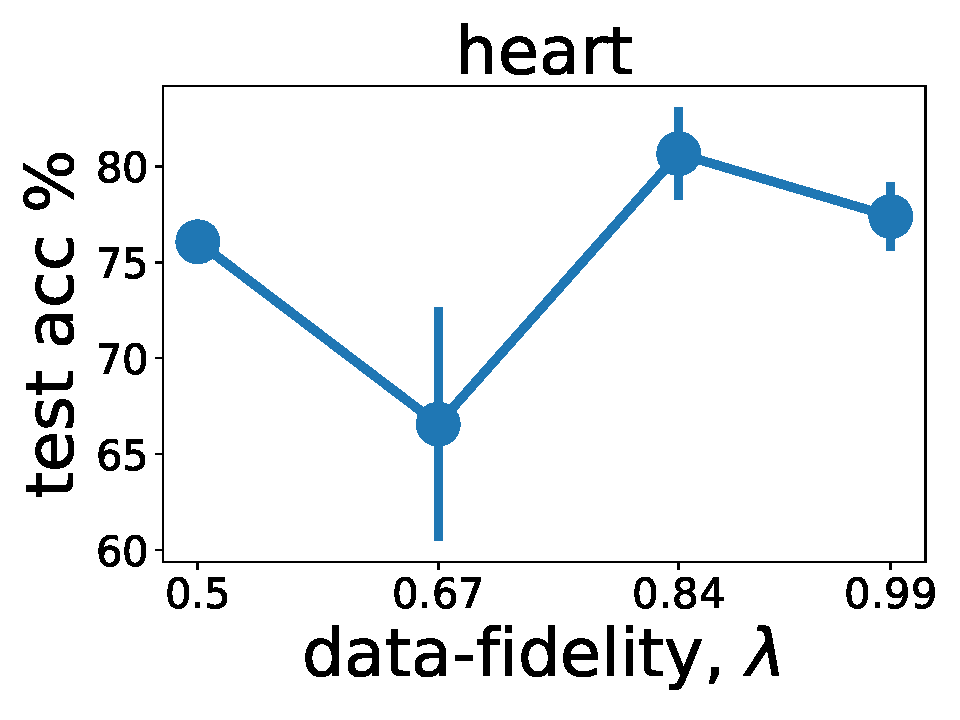
\includegraphics[width=0.27\textwidth]{figures/interpretability/relaxed-cnf/heart_test_accuracy_vary_lambda.pdf}}
	\subfloat
	{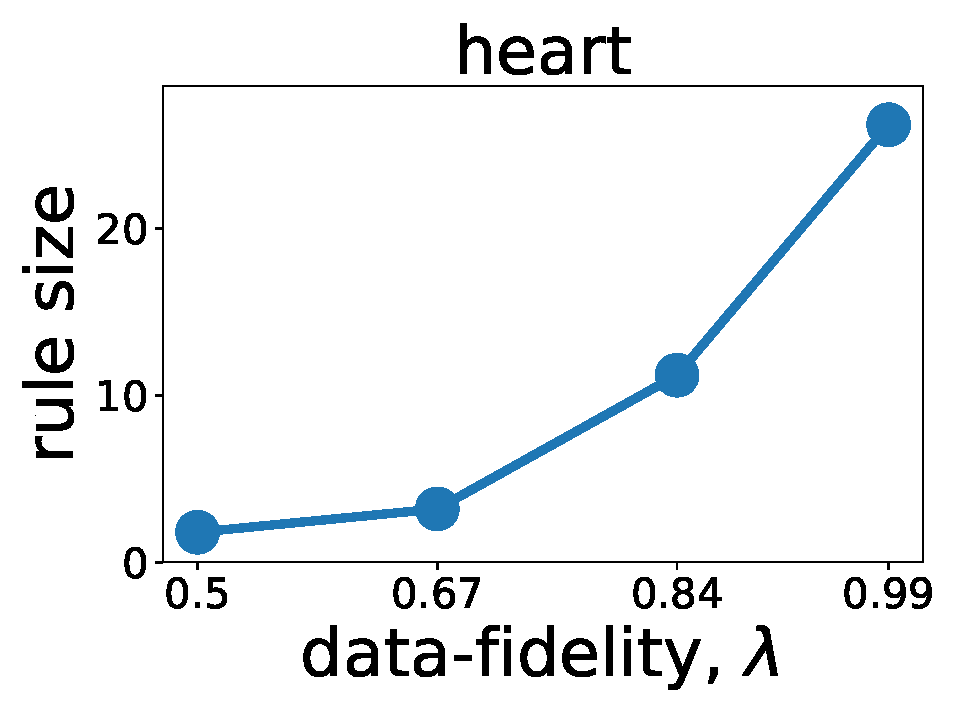
\includegraphics[width=0.27\textwidth]{figures/interpretability/relaxed-cnf/heart_rule_size_vary_lambda.pdf}}
	\subfloat
	{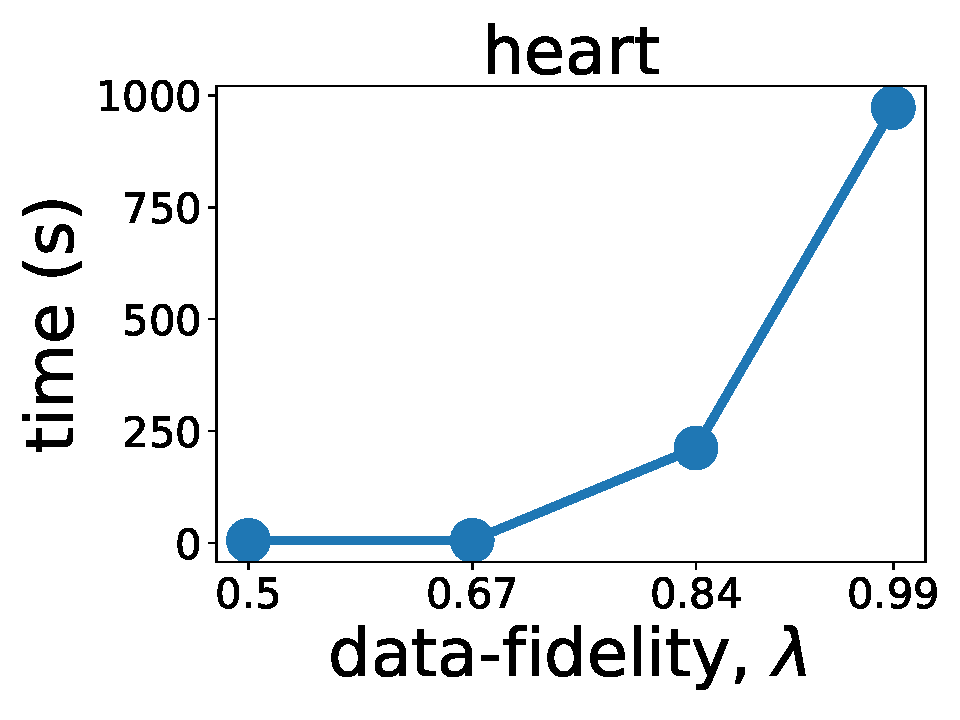
\includegraphics[width=0.27\textwidth]{figures/interpretability/relaxed-cnf/heart_time_vary_lambda.pdf}} 
	\\

	\subfloat
	{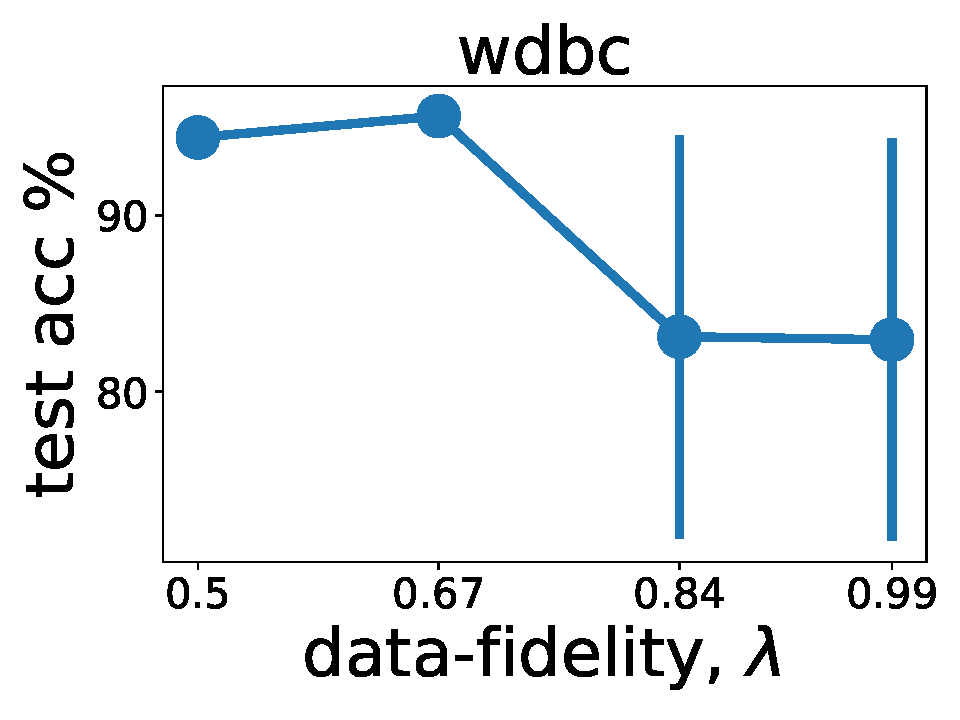
\includegraphics[width=0.27\textwidth]{figures/interpretability/relaxed-cnf/wdbc_test_accuracy_vary_lambda.pdf}}
	\subfloat
	{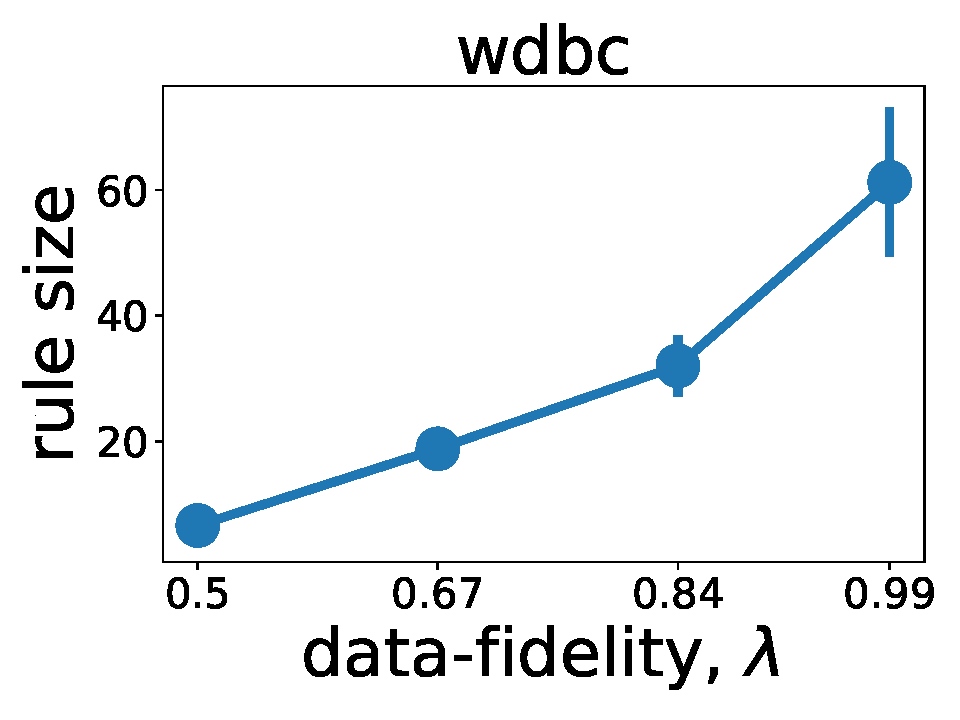
\includegraphics[width=0.27\textwidth]{figures/interpretability/relaxed-cnf/wdbc_rule_size_vary_lambda.pdf}}
	\subfloat
	{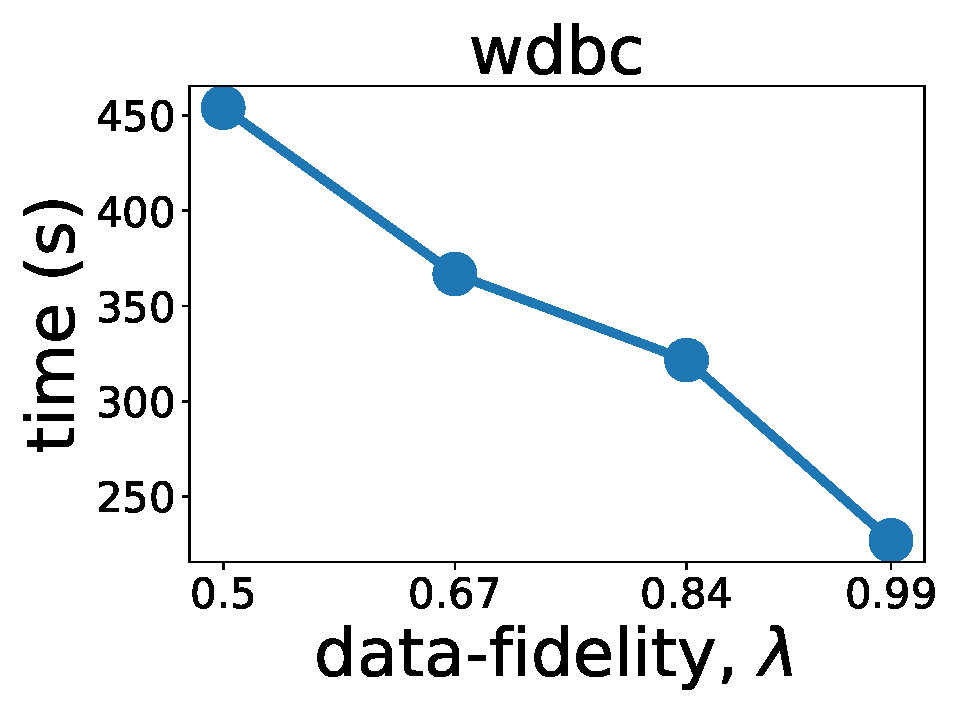
\includegraphics[width=0.27\textwidth]{figures/interpretability/relaxed-cnf/wdbc_time_vary_lambda.pdf}} 
	\\
	
	\subfloat
	{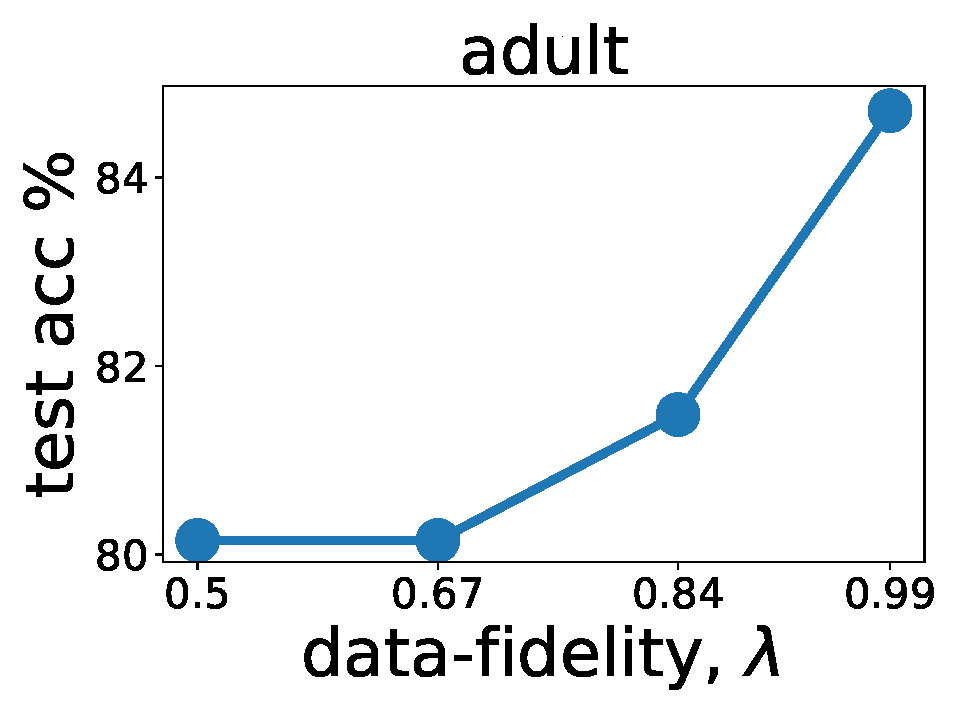
\includegraphics[width=0.27\textwidth]{figures/interpretability/relaxed-cnf/adult_test_accuracy_vary_lambda.pdf}}
	\subfloat
	{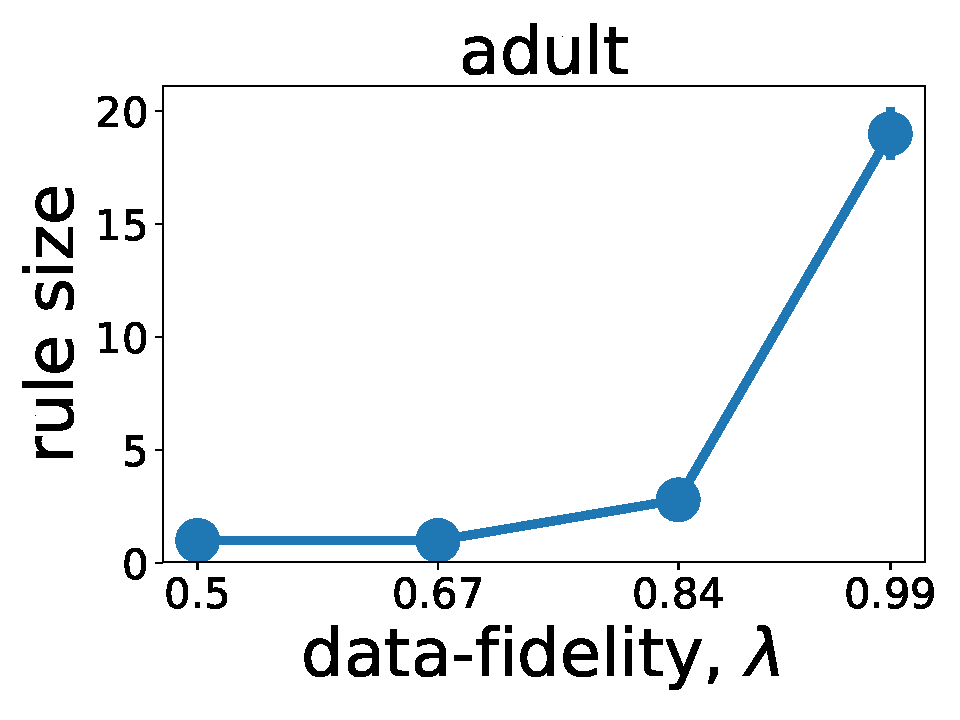
\includegraphics[width=0.27\textwidth]{figures/interpretability/relaxed-cnf/adult_rule_size_vary_lambda.pdf}}
	\subfloat
	{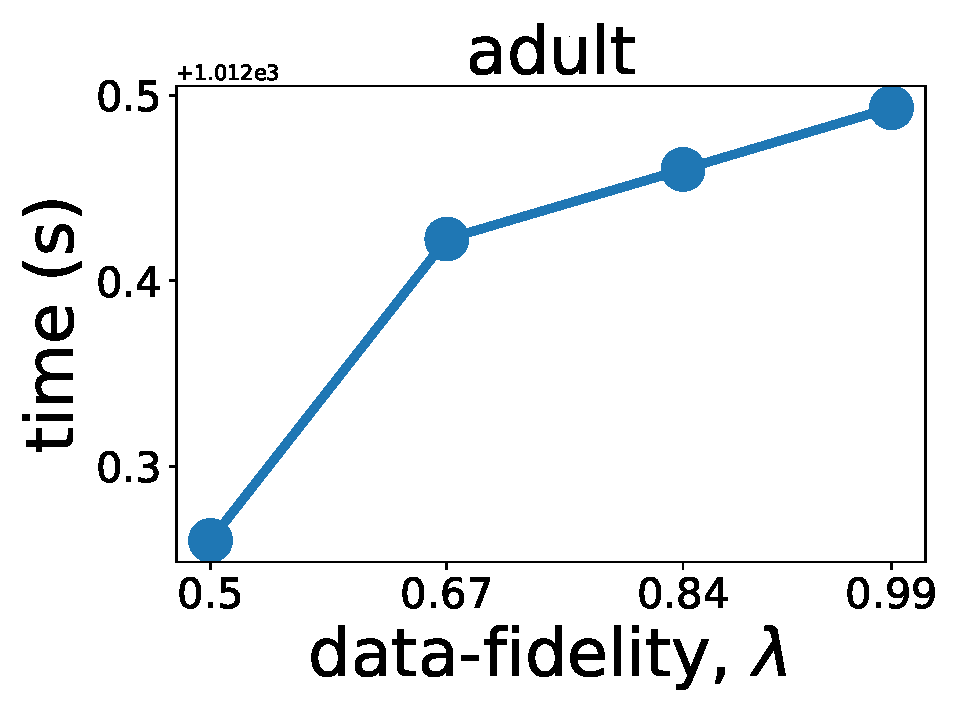
\includegraphics[width=0.27\textwidth]{figures/interpretability/relaxed-cnf/adult_time_vary_lambda.pdf}} 
	\\
	

	\caption[Effect of data-fidelity $ \lambda $ in {\crr}]{Effect of data-fidelity $ \lambda $ on test accuracy, rule-size, and training time in {\crr}. } 
	\label{interpretability_crr_fig:result_lambda}
\end{figure}


\begin{figure}[t]
	\centering
	
	\subfloat
	{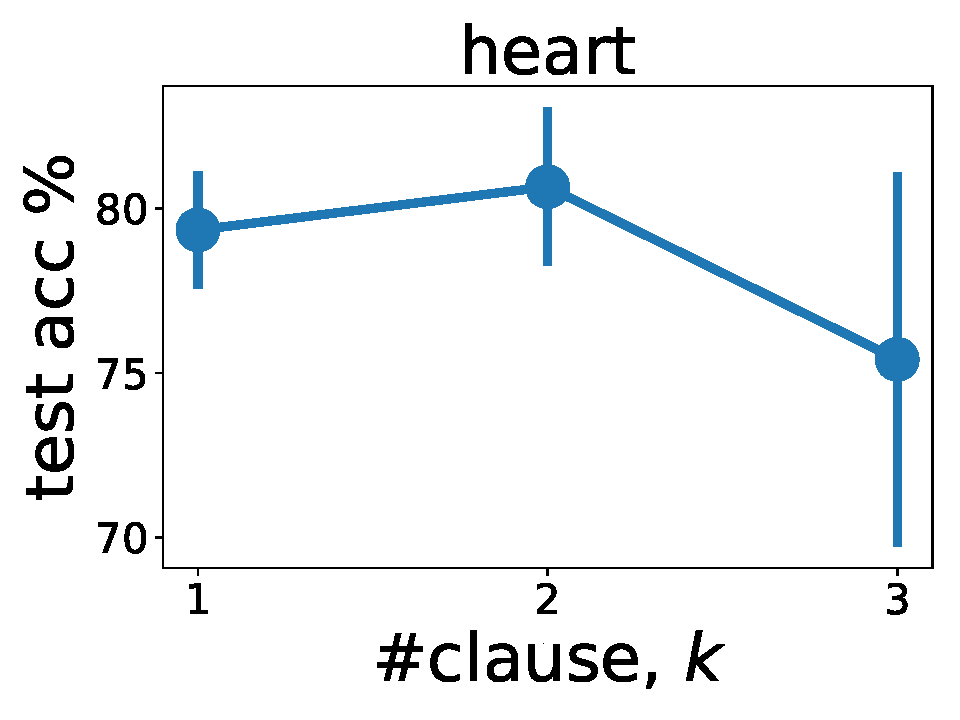
\includegraphics[width=0.27\textwidth]{figures/interpretability/relaxed-cnf/heart_test_accuracy_vary_clause.pdf}}
	\subfloat
	{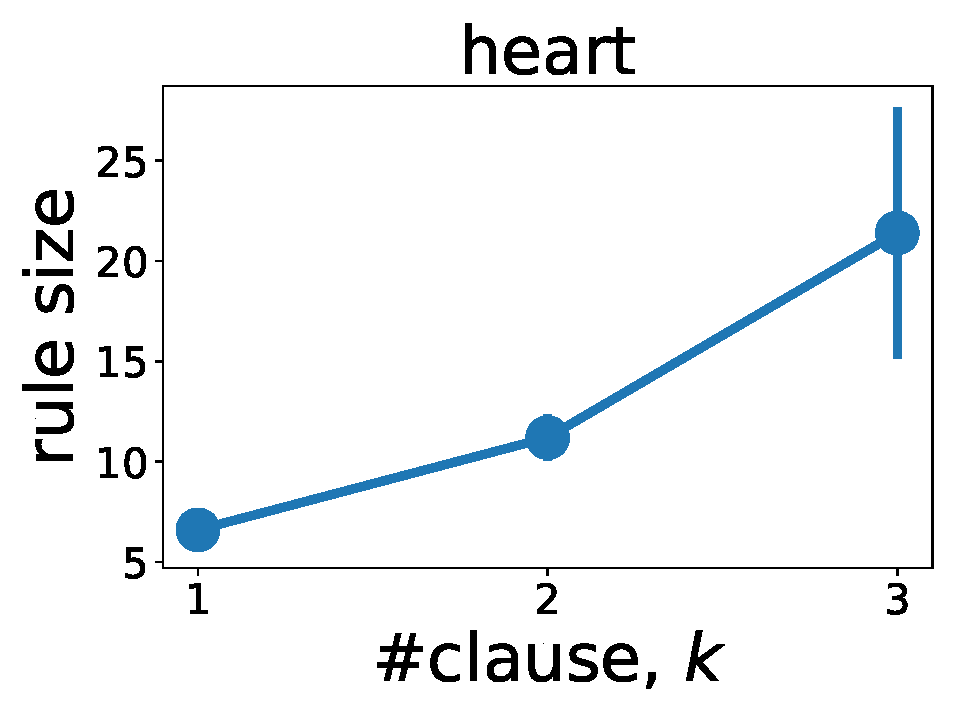
\includegraphics[width=0.27\textwidth]{figures/interpretability/relaxed-cnf/heart_rule_size_vary_clause.pdf}}
	\subfloat
	{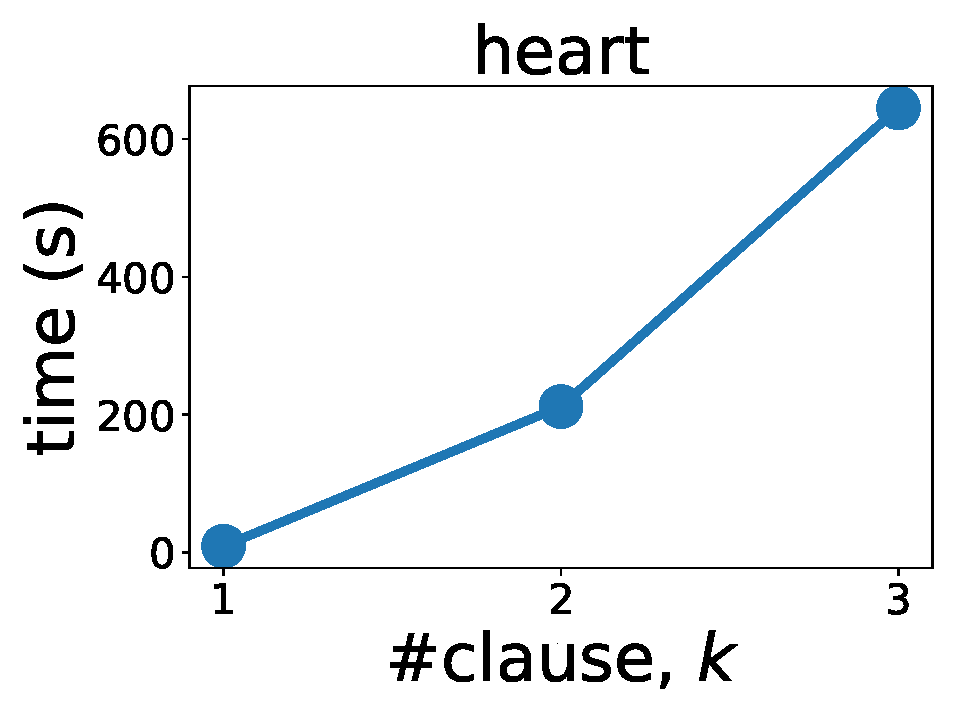
\includegraphics[width=0.27\textwidth]{figures/interpretability/relaxed-cnf/heart_time_vary_clause.pdf}} 
	\\
	
	\subfloat
	{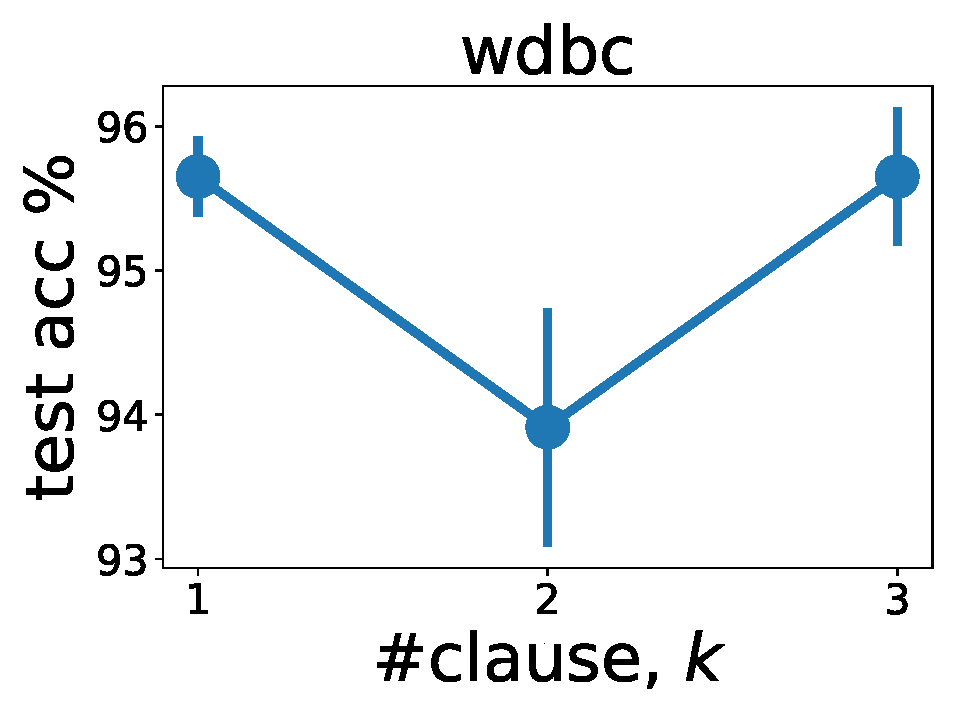
\includegraphics[width=0.27\textwidth]{figures/interpretability/relaxed-cnf/wdbc_test_accuracy_vary_clause.pdf}}
	\subfloat
	{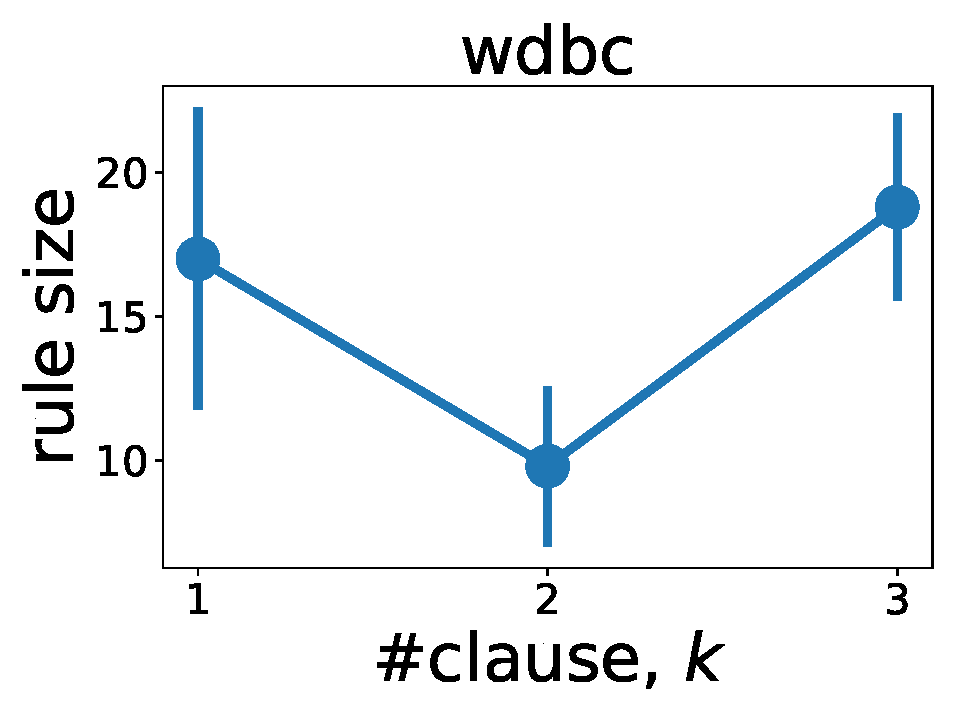
\includegraphics[width=0.27\textwidth]{figures/interpretability/relaxed-cnf/wdbc_rule_size_vary_clause.pdf}}
	\subfloat
	{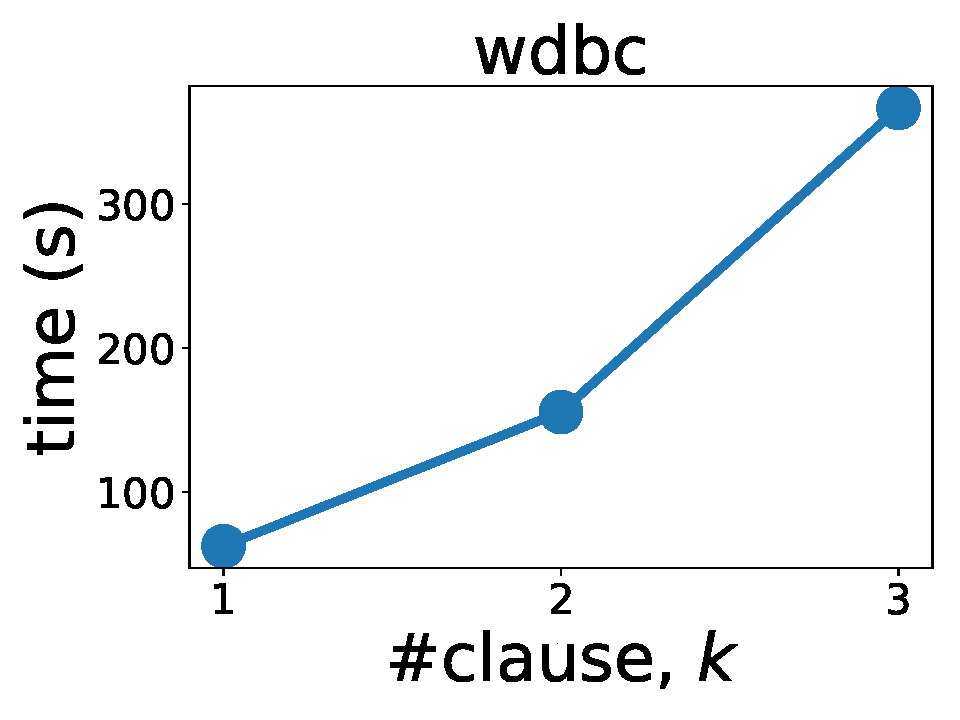
\includegraphics[width=0.27\textwidth]{figures/interpretability/relaxed-cnf/wdbc_time_vary_clause.pdf}} 
	\\
	
	\subfloat
	{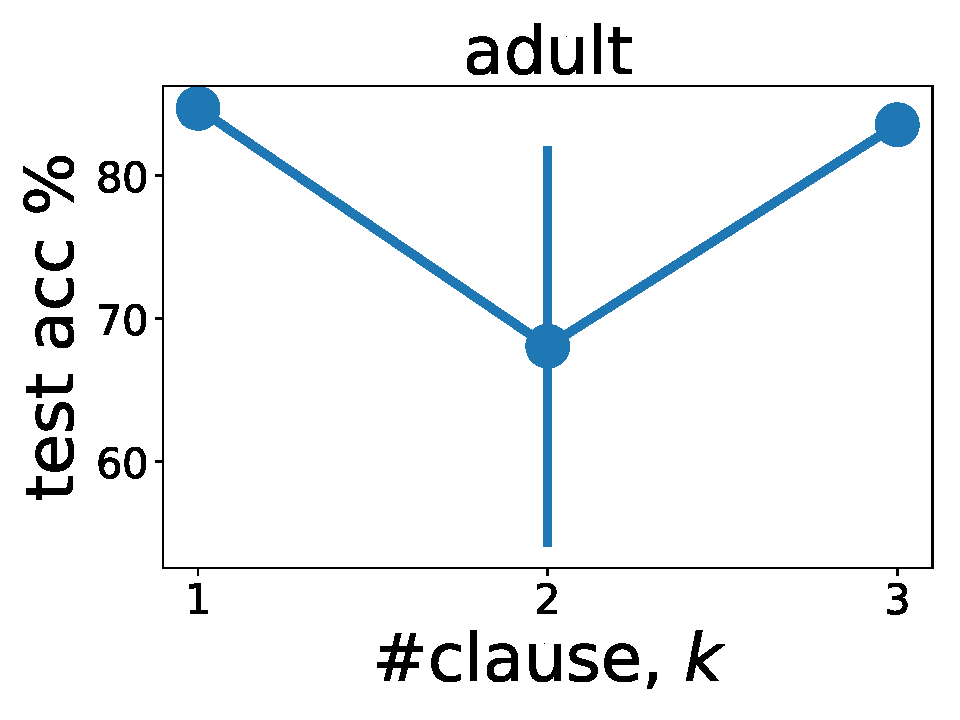
\includegraphics[width=0.27\textwidth]{figures/interpretability/relaxed-cnf/adult_test_accuracy_vary_clause.pdf}}
	\subfloat
	{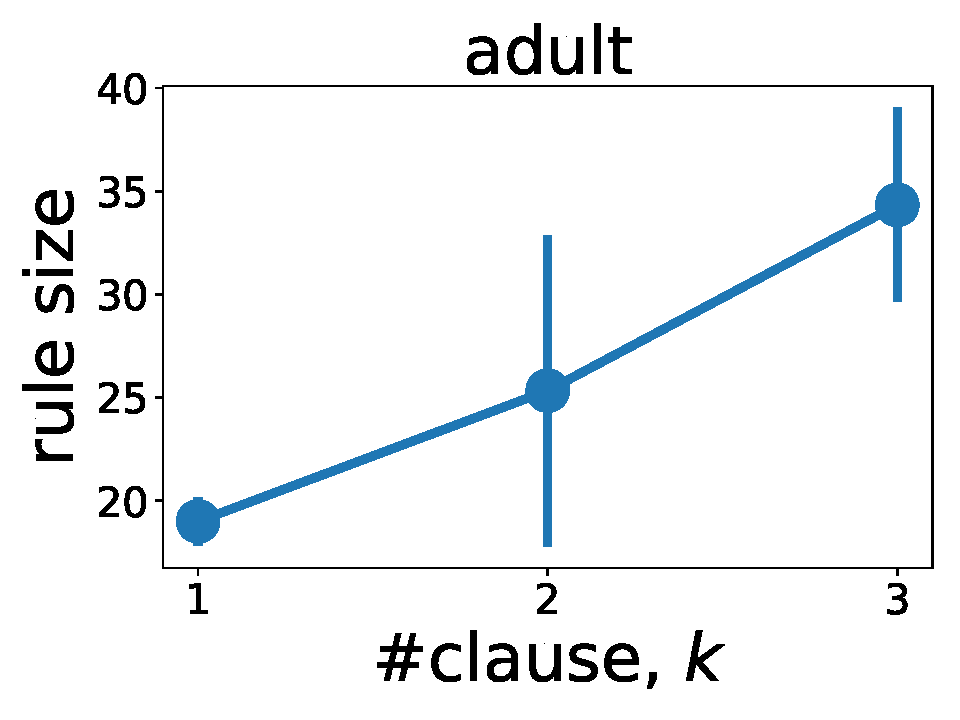
\includegraphics[width=0.27\textwidth]{figures/interpretability/relaxed-cnf/adult_rule_size_vary_clause.pdf}}
	\subfloat
	{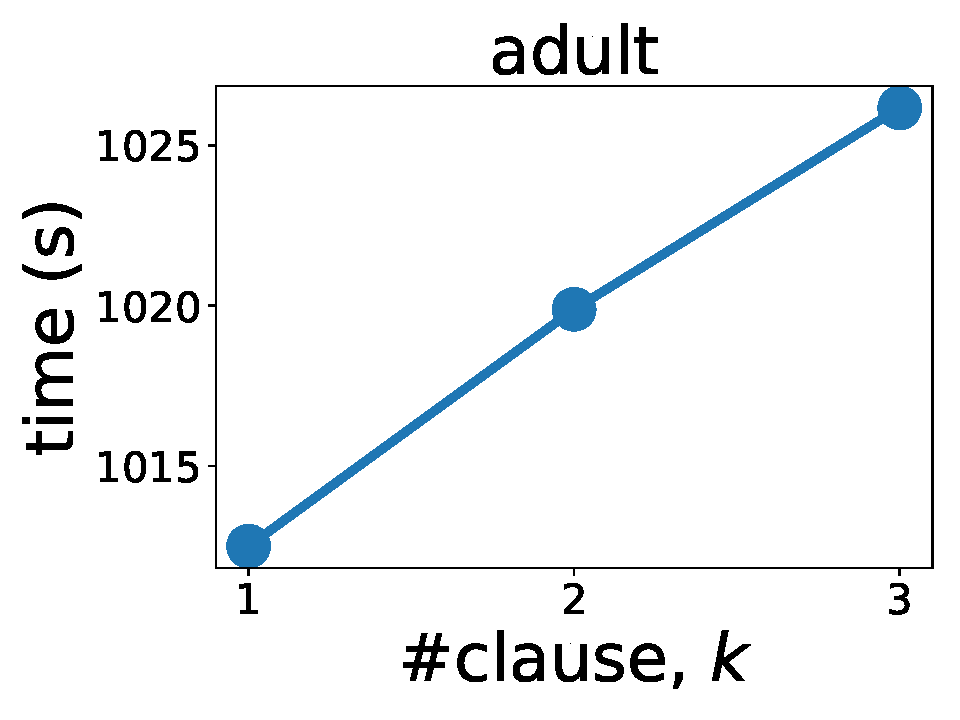
\includegraphics[width=0.27\textwidth]{figures/interpretability/relaxed-cnf/adult_time_vary_clause.pdf}} 
	\\
	
	
	\caption[Effect of the number of clause $ k $ in {\crr}]{Effect of the number of clause $ k $ on test accuracy, rule-size, and training time in {\crr}. } 
	\label{interpretability_crr_fig:result_clause}
\end{figure}



\begin{figure}[t]
	\centering
	
	\subfloat
	{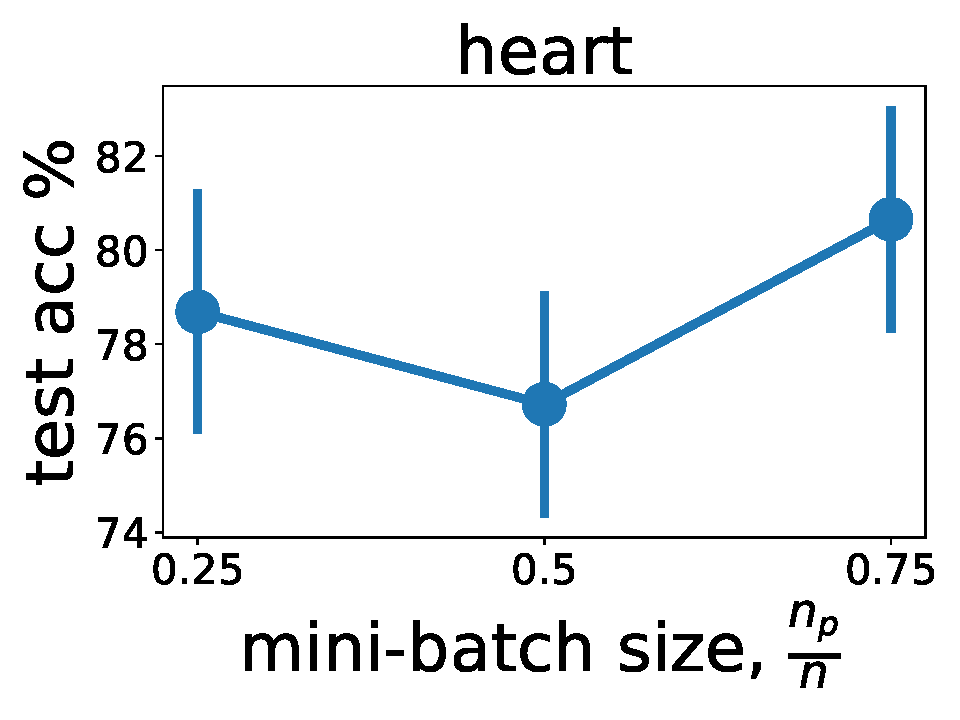
\includegraphics[width=0.27\textwidth]{figures/interpretability/relaxed-cnf/heart_test_accuracy_vary_subsamplesize.pdf}}
	\subfloat
	{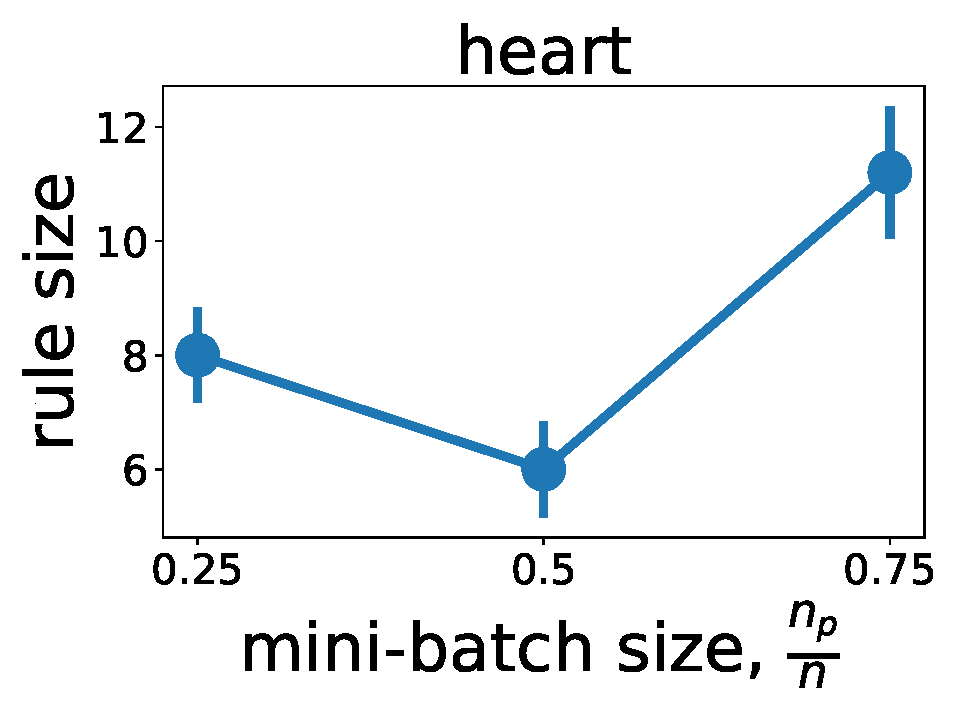
\includegraphics[width=0.27\textwidth]{figures/interpretability/relaxed-cnf/heart_rule_size_vary_subsamplesize.pdf}}
	\subfloat
	{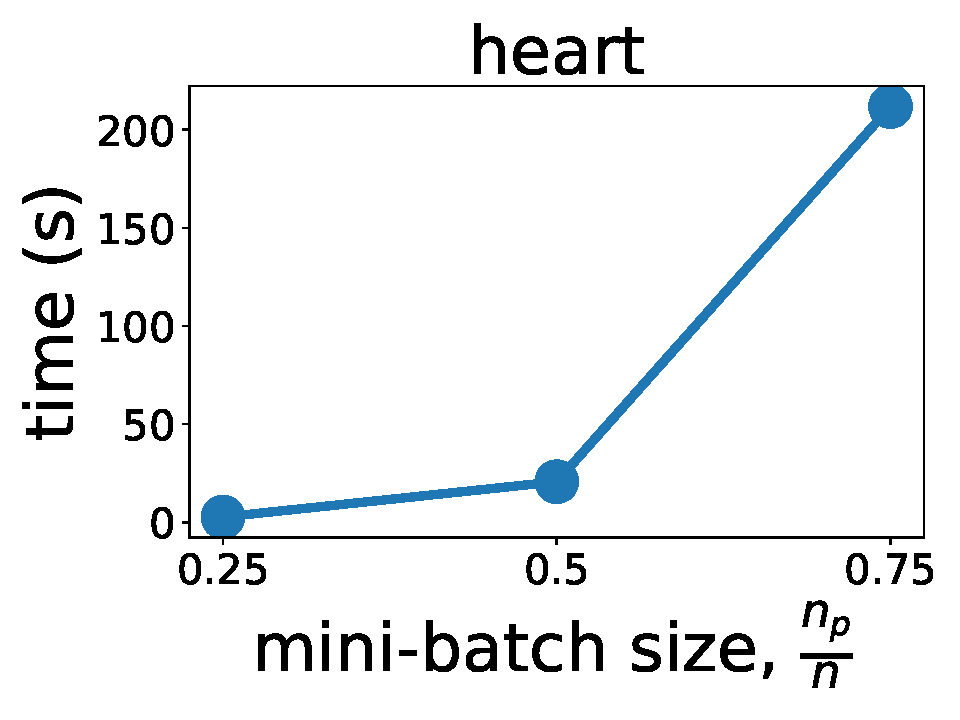
\includegraphics[width=0.27\textwidth]{figures/interpretability/relaxed-cnf/heart_time_vary_subsamplesize.pdf}} 
	\\
	
	\subfloat
	{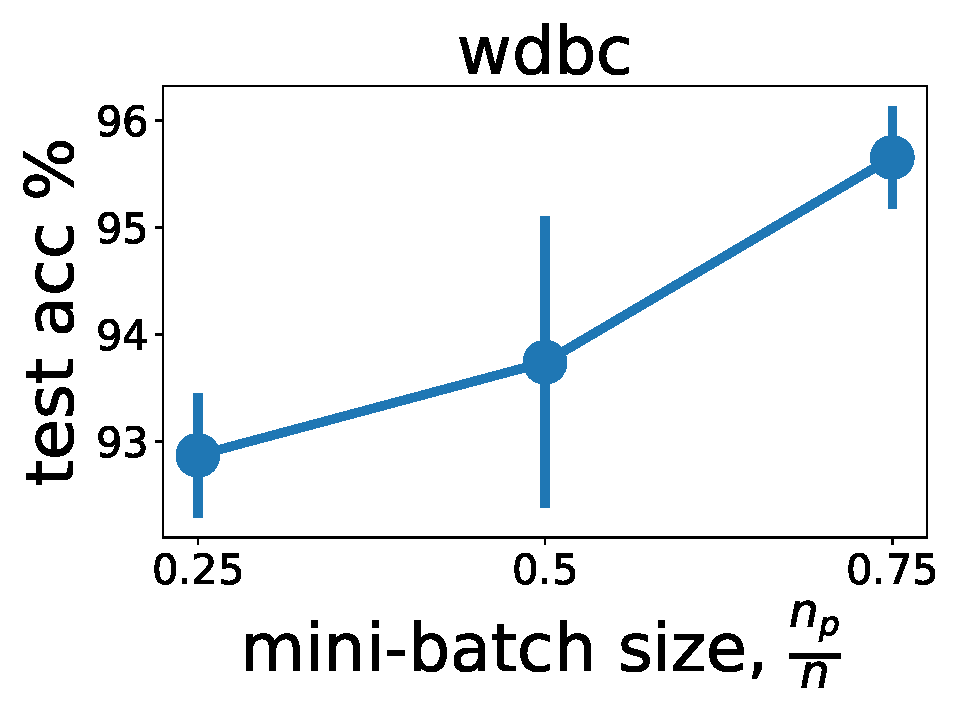
\includegraphics[width=0.27\textwidth]{figures/interpretability/relaxed-cnf/wdbc_test_accuracy_vary_subsamplesize.pdf}}
	\subfloat
	{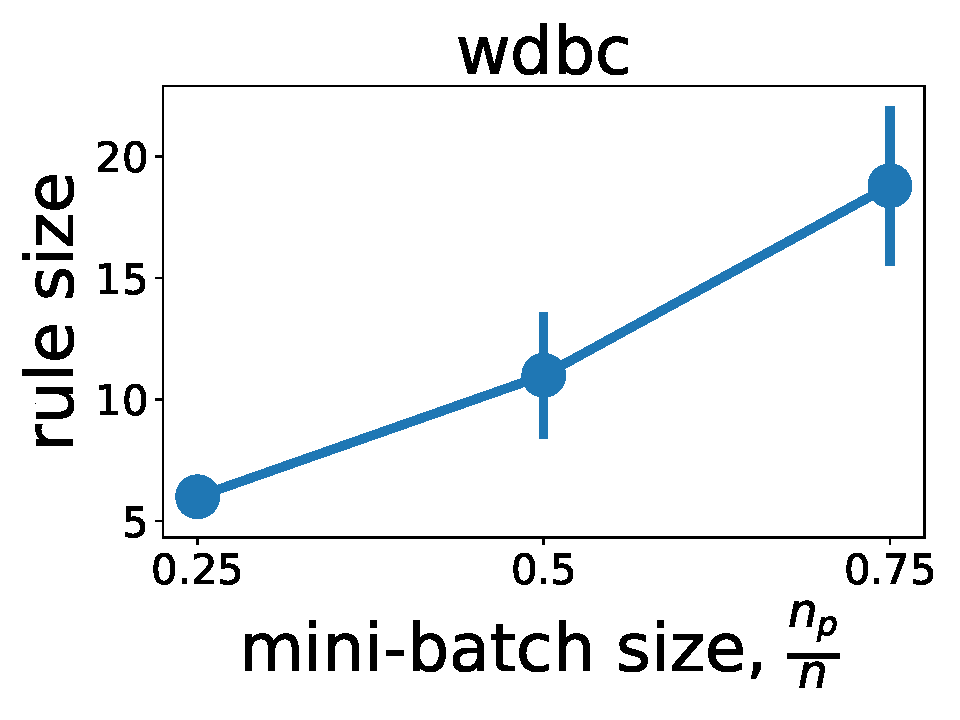
\includegraphics[width=0.27\textwidth]{figures/interpretability/relaxed-cnf/wdbc_rule_size_vary_subsamplesize.pdf}}
	\subfloat
	{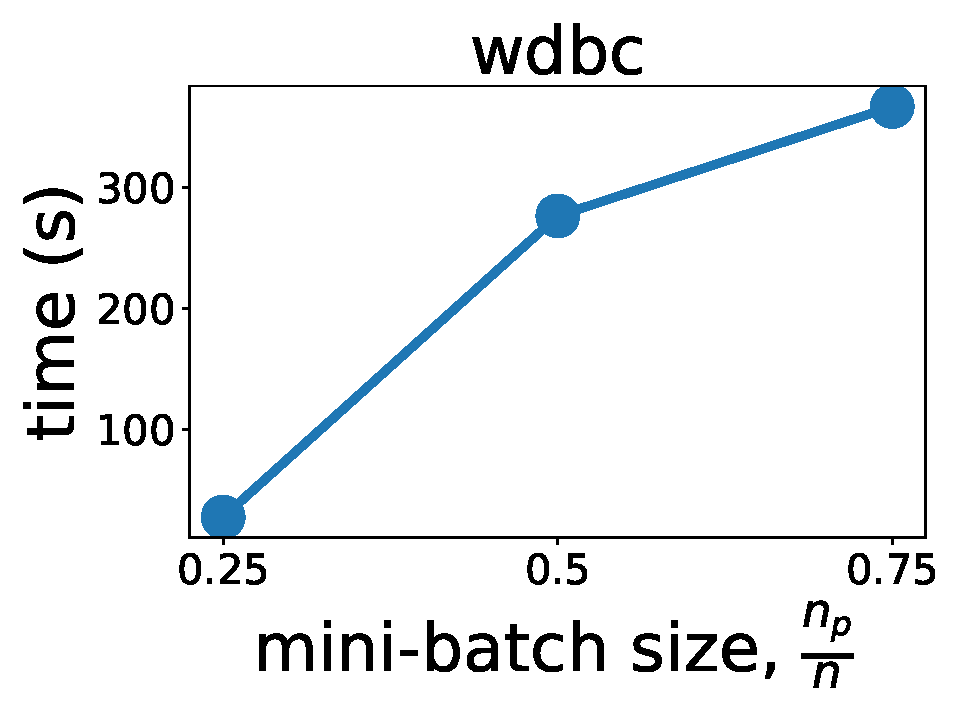
\includegraphics[width=0.27\textwidth]{figures/interpretability/relaxed-cnf/wdbc_time_vary_subsamplesize.pdf}} 
	\\
	
	\subfloat
	{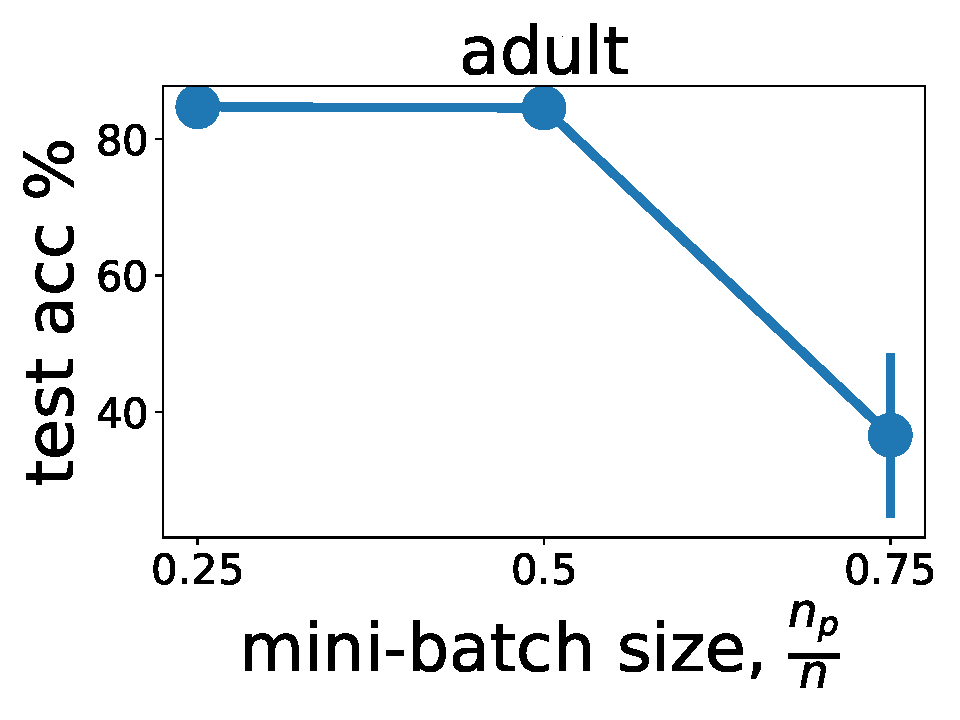
\includegraphics[width=0.27\textwidth]{figures/interpretability/relaxed-cnf/adult_test_accuracy_vary_subsamplesize.pdf}}
	\subfloat
	{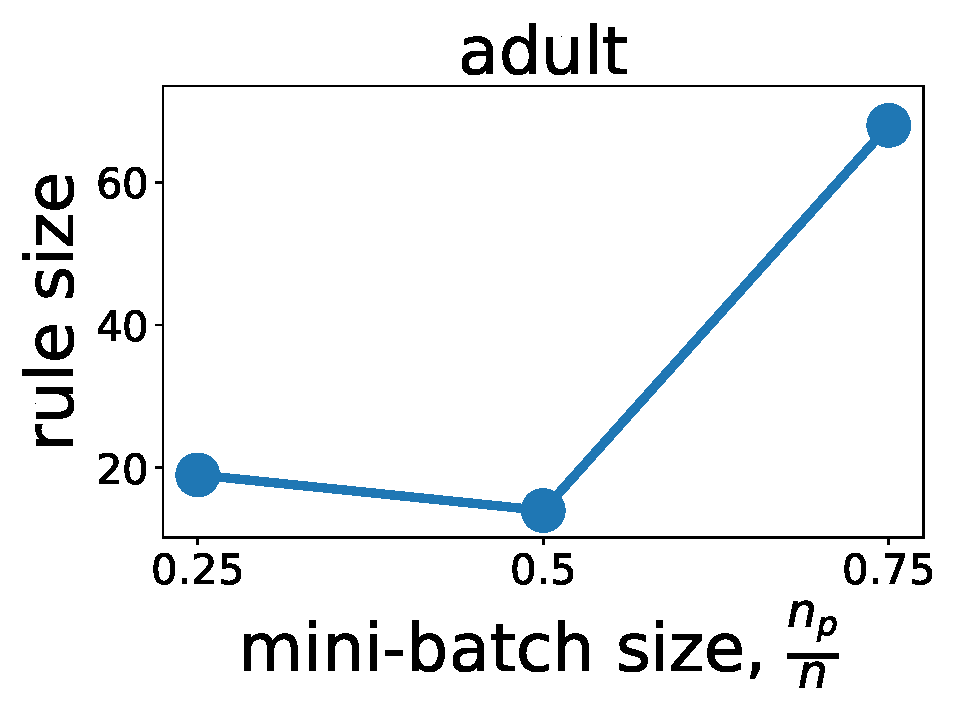
\includegraphics[width=0.27\textwidth]{figures/interpretability/relaxed-cnf/adult_rule_size_vary_subsamplesize.pdf}}
	\subfloat
	{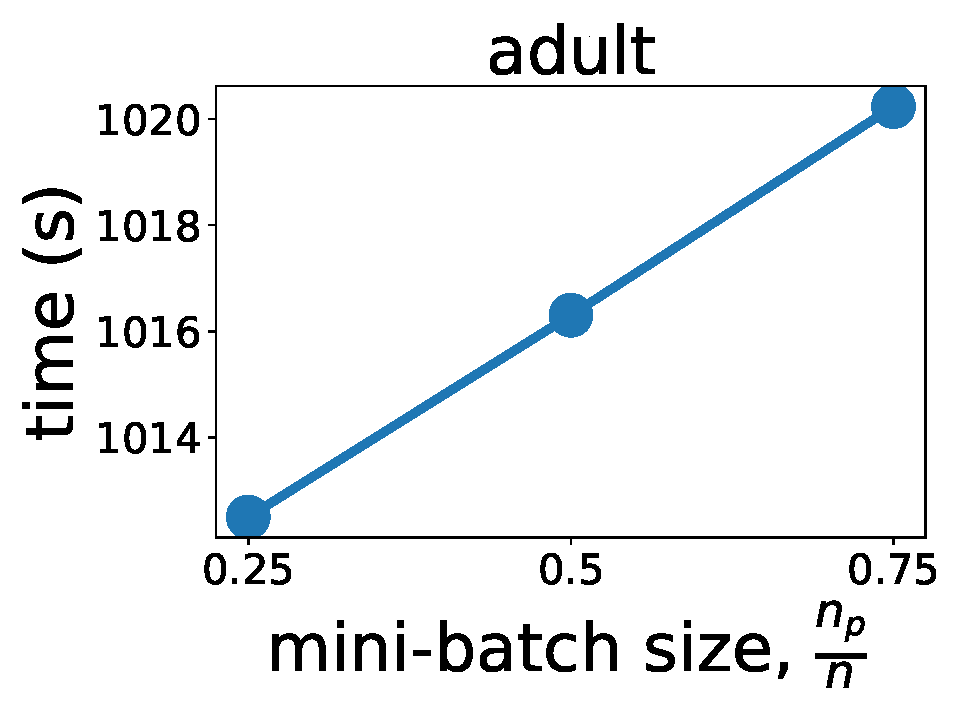
\includegraphics[width=0.27\textwidth]{figures/interpretability/relaxed-cnf/adult_time_vary_subsamplesize.pdf}} 
	\\
	
	
	\caption[Effect of mini-batch size in {\crr}]{Effect of mini-batch size on test accuracy, rule-size, and training time in {\crr}. } 
	\label{interpretability_crr_fig:result_minibatch}
\end{figure}




\begin{figure}[t]
	\centering
	
	\subfloat
	{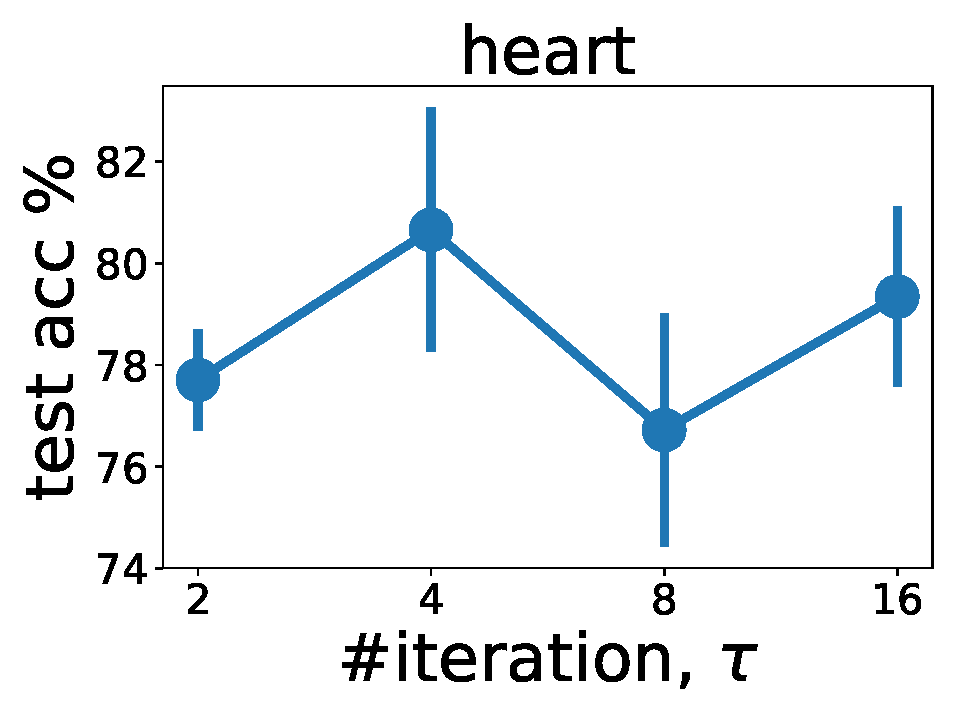
\includegraphics[width=0.27\textwidth]{figures/interpretability/relaxed-cnf/heart_test_accuracy_vary_iteration.pdf}}
	\subfloat
	{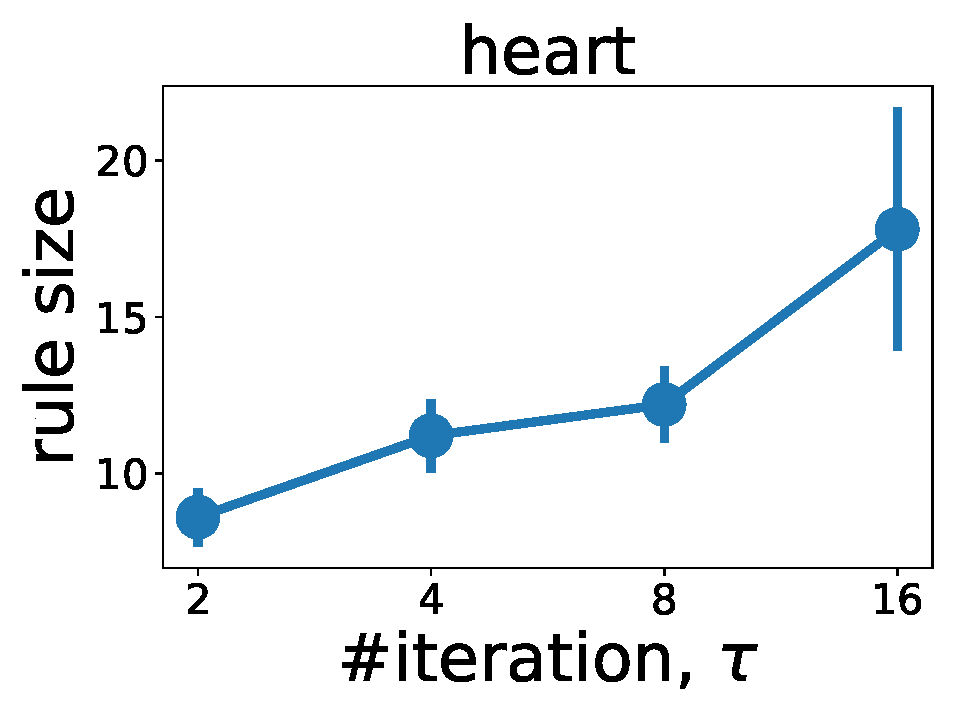
\includegraphics[width=0.27\textwidth]{figures/interpretability/relaxed-cnf/heart_rule_size_vary_iteration.pdf}}
	\subfloat
	{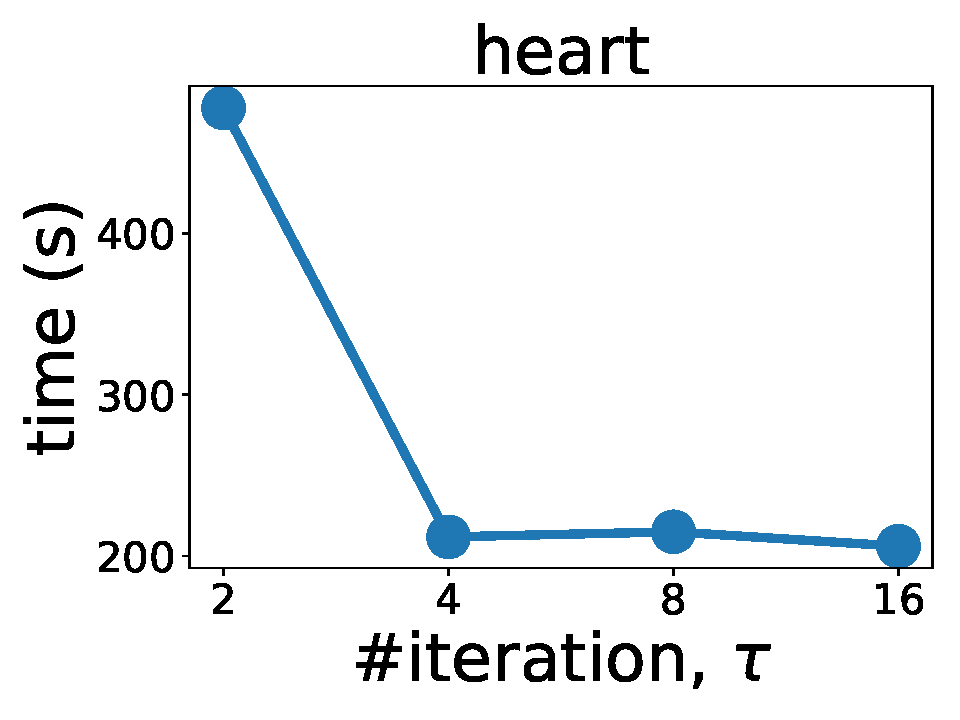
\includegraphics[width=0.27\textwidth]{figures/interpretability/relaxed-cnf/heart_time_vary_iteration.pdf}} 
	\\
	
	\subfloat
	{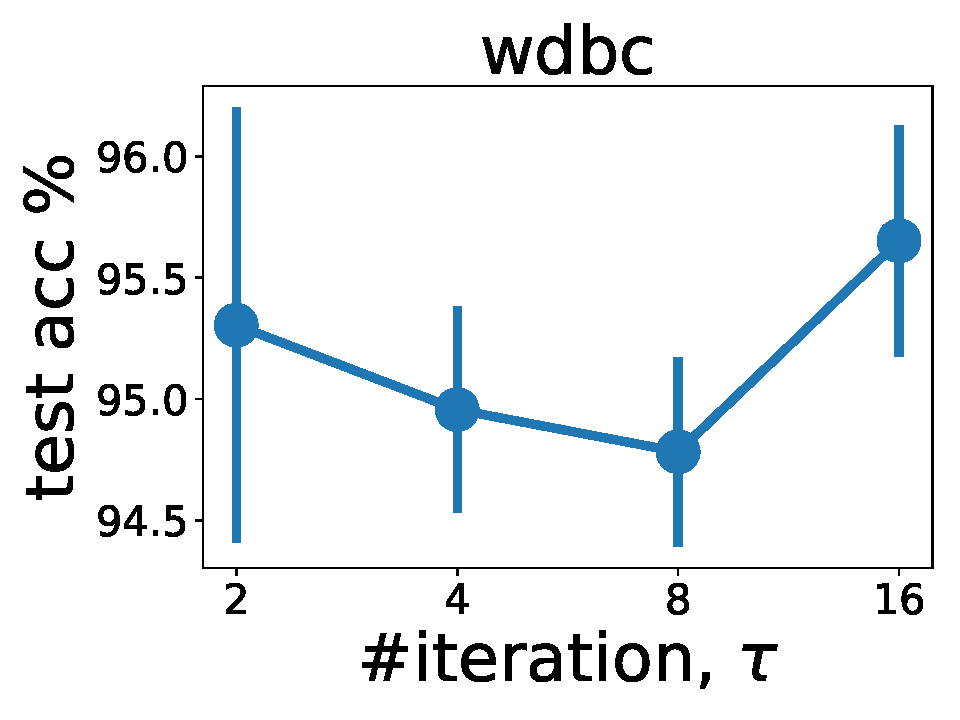
\includegraphics[width=0.27\textwidth]{figures/interpretability/relaxed-cnf/wdbc_test_accuracy_vary_iteration.pdf}}
	\subfloat
	{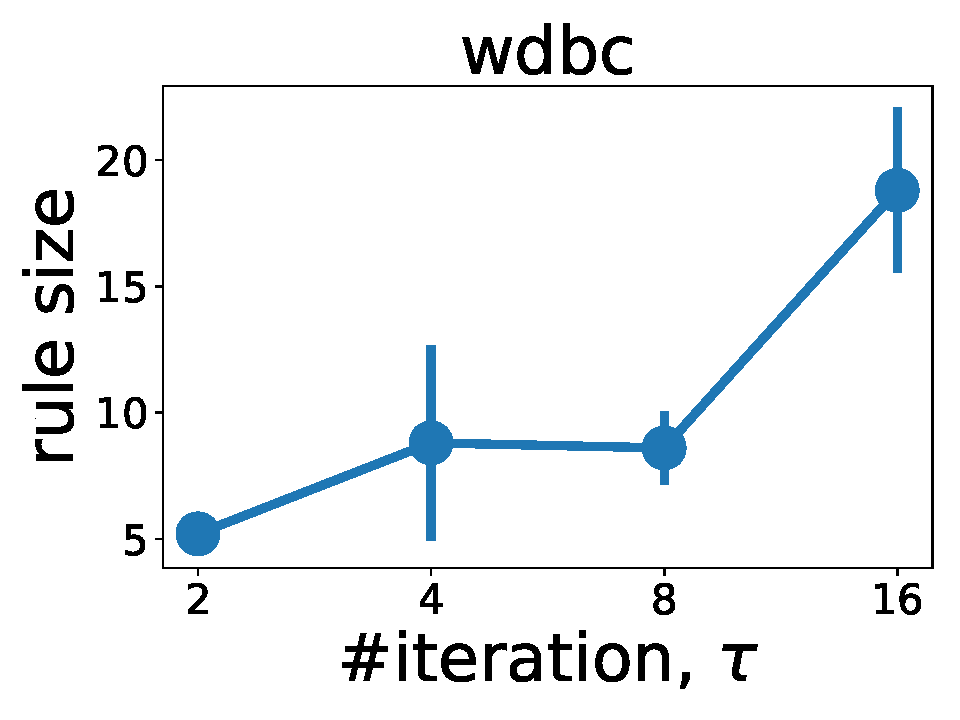
\includegraphics[width=0.27\textwidth]{figures/interpretability/relaxed-cnf/wdbc_rule_size_vary_iteration.pdf}}
	\subfloat
	{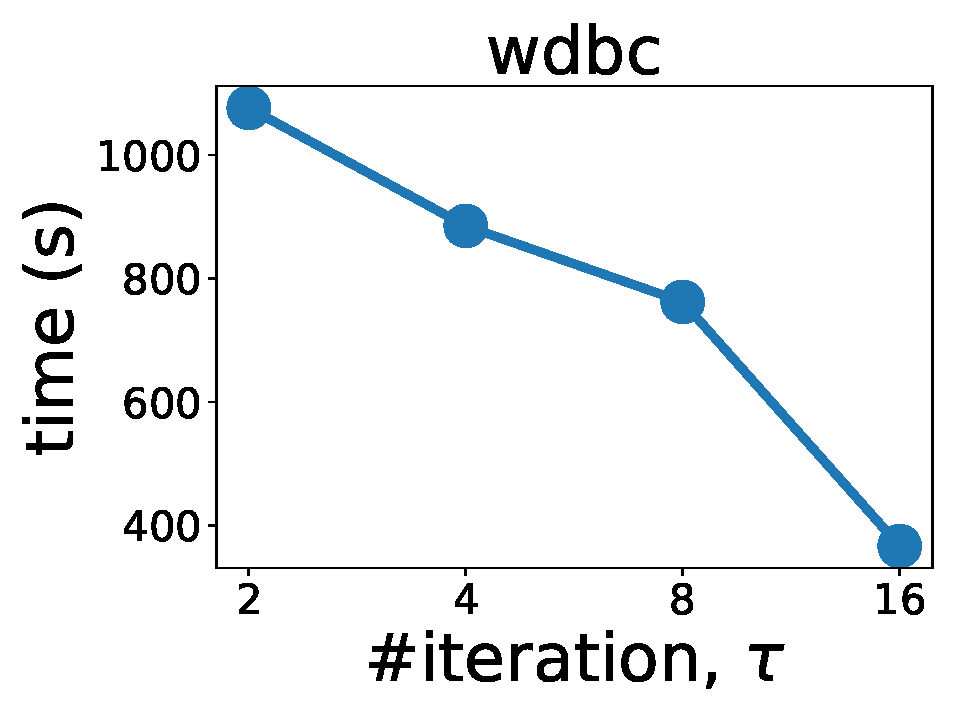
\includegraphics[width=0.27\textwidth]{figures/interpretability/relaxed-cnf/wdbc_time_vary_iteration.pdf}} 
	\\
	
	\subfloat
	{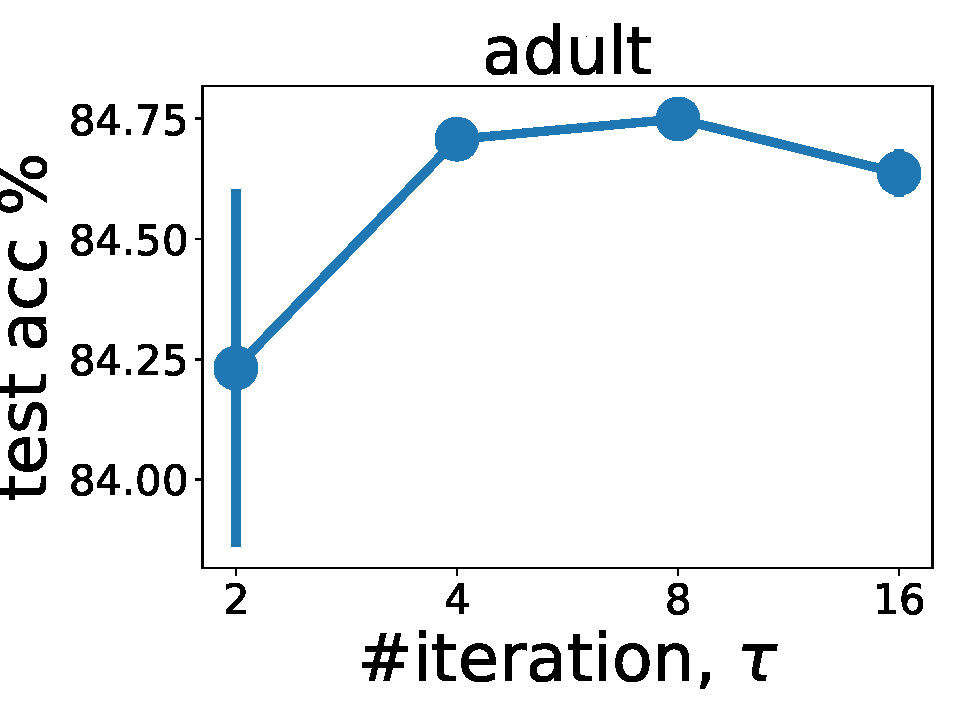
\includegraphics[width=0.27\textwidth]{figures/interpretability/relaxed-cnf/adult_test_accuracy_vary_iteration.pdf}}
	\subfloat
	{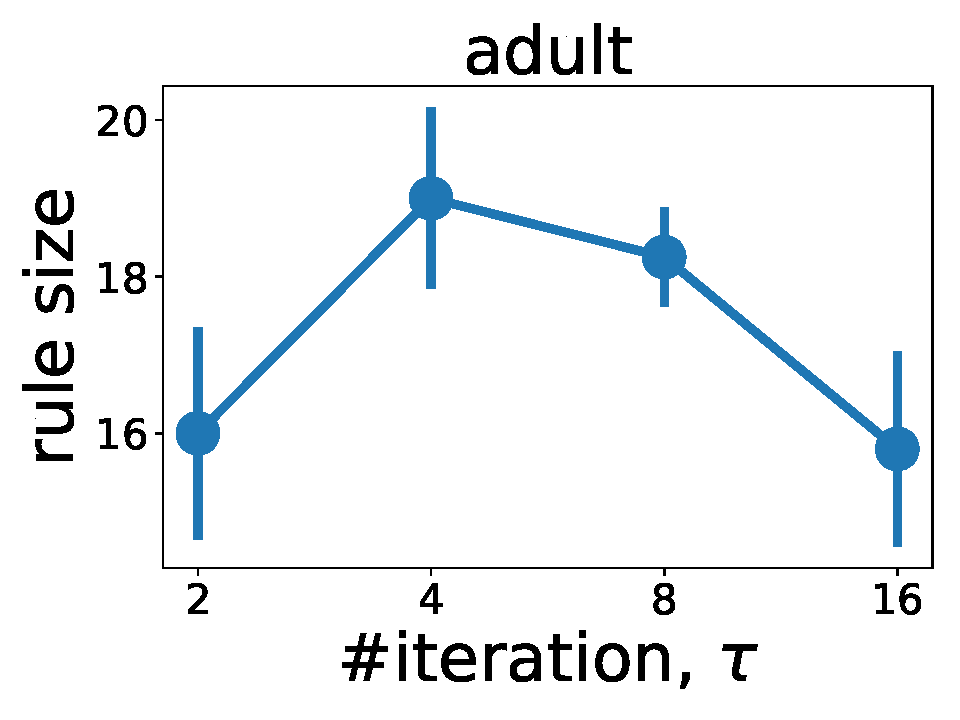
\includegraphics[width=0.27\textwidth]{figures/interpretability/relaxed-cnf/adult_rule_size_vary_iteration.pdf}}
	\subfloat
	{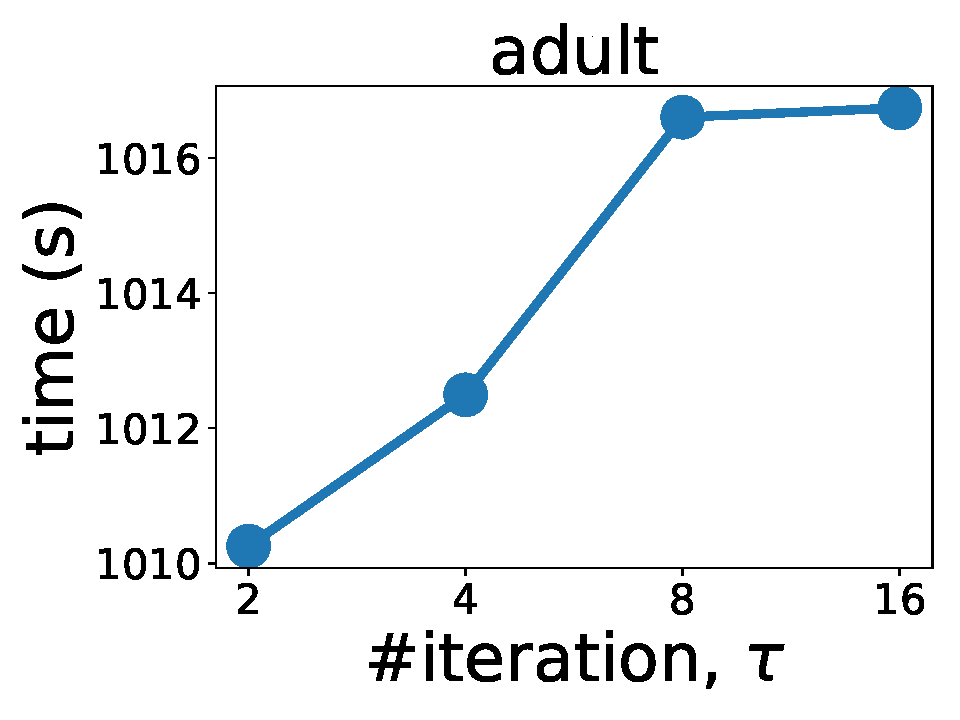
\includegraphics[width=0.27\textwidth]{figures/interpretability/relaxed-cnf/adult_time_vary_iteration.pdf}} 
	\\
	
	
	\caption[Effect of the number of iterations in {\crr}]{Effect of the number of iterations on test accuracy, rule-size, and training time in {\crr}. } 
	\label{interpretability_crr_fig:result_iteration}
\end{figure}





	

	\subsubsection*{Varying Model Parameters: }
	\label{interpretability_crr_sec:model_parameters}
	In Figure~\ref{interpretability_crr_fig:result_lambda},~\ref{interpretability_crr_fig:result_clause}, ,~\ref{interpretability_crr_fig:result_minibatch}, and~\ref{interpretability_crr_fig:result_iteration}, we demonstrate the effect of varying the hyper-parameters of {\crr}. To understand the effect of a single hyper-parameter, we fix the values of other hyper-parameters to a default choice where the default choice results in the most accurate rule. 
	 

	\paragraph{Varying data-fidelity parameter ($ \lambda $):} In Figure~\ref{interpretability_crr_fig:result_lambda}, as we increase data-fidelity parameter $ \lambda $ in the objective function in Eq.~\ref{interpretability_crr_eq:ilp_obj} and Eq.~\ref{interpretability_crr_eq:ilp_inc}, more priority is given to the prediction accuracy than the sparsity of the rules.  In most of the datasets, we similarly observe an increase in accuracy  and also an increase in the size of the rules when $ \lambda $ is higher. This suggests that improved interpretability can often come at a  minor cost in accuracy.  In addition, we  find an increase in training time for most of the datasets indicating that the MILP query usually takes a longer time to find the solution when more priority is given on the prediction accuracy.  
	

	
	\paragraph{Varying the number of clauses ($ k $): }
	In Figure~\ref{interpretability_crr_fig:result_clause}, as we increase  $ k $, {\crr} allows the generated rules to capture the variance in the given dataset more effectively, that results in higher  accuracy in most of the datasets. The  rule-size also increases as we learn more clauses. In addition, the training time  increases, that can be reasoned by the fact that the number of constraints in the MILP formulation is linear with $ k $. Thereby, the number of clauses $ k $ provides a control over the accuracy of the generated rule and training time. 
	 
	 
	 
	\paragraph{Relative size of the mini-batch:} In Figure~\ref{interpretability_crr_fig:result_minibatch}, we vary the relative size of the mini-batch $ \frac{n_p}{n} $ to observe its effect on the accuracy and the size of the rules. In most datasets,  the accuracy increases when more samples are considered in the mini-batch, costing higher   training time.  Moreover, the size of the generated rule increases as $ \frac{n_p}{n} $ increases, that can be supported by the increase  in the variance of the samples in the mini-batch.
	
	%	%%\vspace{-3pt}
	\paragraph{Varying the number of iterations ($ \tau $):}   
	In Figure~\ref{interpretability_crr_fig:result_iteration}, as we allow more iterations in the learning process, we find an increase in accuracy in most datasets. The training time also increases with $ \tau $ because {\crr} is required to solve in total $ \tau $ queries. We also observe an increase in rule-size in most datasets. The reason is that the objective function in the incremental mini-batch approach in Eq.~\ref{interpretability_crr_eq:ilp_inc} does not put a restriction on the size of the rules, rather on the change of rules in consecutive iterations.  In addition, the learned values of the thresholds $ \eta_c$ and $ \eta_l $  in one iteration are not carried to the MILP query in the next iteration, that may cause an increase of rule-size. 
	

	



	
	
